\documentclass[10pt,a4paper]{article}

%double si on veut une version prof et une version élève. simple si on veut une seule version.
\newcommand{\buildmode}{double}

\InputIfFileExists{version.tex}{}{}
% Version (définie par le script)
\providecommand{\version}{eleve}

\usepackage{feuilleactivite}

%%%à modifier à chaque fois

\renewcommand{\niveau}{2nde}
\renewcommand{\chapitre}{Equations produit nul}
\renewcommand{\numchap}{0.4} 
\renewcommand{\theme}{Fonctions}

\begin{document}

\prof{
    Motivation : \begin{itemize}
        \item Dans de nombreux cas, on est amené à résoudre des équations du type \(f(x) = 0\), par exemple, fonction bénéfice
        \item C'est des équations qui sont souvent un peu plus simples à résoudre. Et on peut toujours se ramener à des équations du type \(f(x) = 0\). Exemple : \(x^2-3x = 12\) et \(x^2-3x-12 = 0\) sont équivalentes.
        \item Pourquoi elles sont plus simples à résoudre ? Exemple avec les équations produit nul.
        \item En vrai, surtout demander à Étienne comment il fait.
    \end{itemize}
    Pas convaincu par ma fiche d'exos en vrai
}
\begin{objectifs}
\begin{itemize}
    \item Savoir résoudre des problèmes à l'aide d'équation produit nul.
    \item Se ramener à une équation produit nul pour résoudre un problème.
\end{itemize}
\end{objectifs}

\begin{multicols}{2}
\begin{exo}[][]
Résoudre les équations produit nul suivantes :\begin{tasks}(2)
    \task \((x-4)(2x+5)=0\)
    \task \((2x+1)(5x-3)=0\)
    \task \((2x+1)x=0\)
    \task \((x+3)^2=0\)
\end{tasks}
\end{exo}

\begin{exo}[][]

    Relier chaque fonction ci-dessous à sa représentation graphique : 

    \hspace{-1cm}\begin{tabular}{*{4}{c}}
        \(f(x) = x(x-5)\) &
        \(g(x) = -\dfrac{1}{2}(x-1)(2x+10)\) &
        \(g(x) = (x+1)(x+5)\) \\
        \(\bullet\) & \(\bullet\) & \(\bullet\)  \vspace{0.6cm} \\
        \(\bullet\) & \(\bullet\) & \(\bullet\) \\
        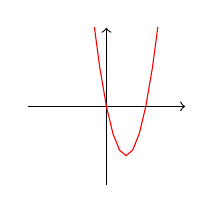
\begin{tikzpicture}[scale=0.1]
            \clip(-10,-10) rectangle (10,10);
            \draw[->] (-10,0)--(10,0);
            \draw[->] (0,-10)--(0,10);
             \draw[color=red, domain=-10:10]    plot (\x,{\x*(\x-5)});
        \end{tikzpicture} &
        \begin{tikzpicture}[scale=0.1]
            \clip(-10,-10) rectangle (10,10);
            \draw[->] (-10,0)--(10,0);
            \draw[->] (0,-10)--(0,10);
             \draw[color=red, domain=-10:10]    plot (\x,{(\x+1)*(\x+5)});
        \end{tikzpicture} &
        \begin{tikzpicture}[scale=0.1]
            \clip(-20,-10) rectangle (10,10);
            \draw[->] (-10,0)--(10,0);
            \draw[->] (0,-10)--(0,10);
             \draw[color=red, domain=-10:10]    plot (\x,{-(\x-1)*(2*\x+10)/2});
        \end{tikzpicture}
    \end{tabular}
\end{exo}

\begin{exo}[Vrai ou faux][]

L'affirmation suivante est-elle vraie ou fausse ? Vous justifierez votre réponse. \medbreak

"L'équation \(x(x+1)(3x+2)\) admet trois solutions sur l'intervalle \([0\ ;\ +\infty[\)"
\end{exo}

\begin{exo}
    \begin{enumerate}
        \item Développer l'expression \(-2(x+10)(-4x+5)\)
        \item En déduire les solutions de l'équation \(8x^2+70x = 50\)
    \end{enumerate}
\end{exo}

\begin{exo}[][]
    Une entreprise produit et vend des casquettes. Pour \(x\) milliers de casquettes vendues le bénéfice en milliers d'euros se calcule par \(B(x) = -x^2+4x-3\).
    \begin{enumerate}
        \item \begin{enumerate}
            \item Rappeler la définition du bénéfice.
            \item Quel sera le bénéfice pour 1 000 casquettes vendues ?
        \end{enumerate}
        \item \begin{enumerate}
            \item Développer l'expression \(-(x-1)(x-4)\).
            \item En déduire quand l'entreprise fera un bénéfice nul.
        \end{enumerate}
        \item \begin{enumerate}
            \item Développer l'expression \(-(x-2)^2\)
            \item En déduire quand l'entreprise fera un chiffre d'affaire égal à 1 000 euros.
        \end{enumerate}
        \item Tracer la fonction \(B\) entre 0 et 5. Vous verifierez ainsi si vos résultats sont justes.
    \end{enumerate}
\end{exo}

\begin{exo}[QCM][appro]
    \begin{enumerate}
        \item L'équation \((x-2)(2x-4)(3x-6)=0\) admet \begin{tasks}(2)
            \task Une solution
            \task Deux solutions
            \task Trois solutions
            \task Cela dépend de la valeur de \(x\)
        \end{tasks}
        \item Voici la représentation graphique d'une fonction \(g\) :
        
                \begin{tikzpicture}[yscale=0.1,xscale=0.7]
            \clip(-2,-10) rectangle (10,10);
            \draw[->] (-2,0)--(3.5,0);
            \draw[->] (0,-10)--(0,10);
             \draw[color=red, domain=-3:4]    plot (\x,{(\x-3)*(\x*\x+\x+1)});
            \draw (3,1)--(3,-1) node[below] {3};
        \end{tikzpicture}

        La seule formule possible pour \(g\) est 

        \hspace{-1cm}\begin{minipage}{0.5\textwidth}
        \begin{tasks}(2)
            \task \(g(x)  (x+3)(2x-2)\)
            \task \(g(x)  (3x-1)^2\)
            \task \(g(x)  x^3-3x^2-3x-3\)
            \task \(g(x)  x^3-2x^2-2x-3\)
        \end{tasks}
        \end{minipage} \vspace{0.1cm}

        \item L'équation \((mx+4)(x+m)=0\), d'inconnue \(x\) admet une seule solution si :\begin{tasks}(2)
            \task \(m=1\)
            \task \(m=-1\)
            \task \(m=2\)
            \task \(m=-2\)
        \end{tasks}
    \end{enumerate}
\end{exo}

\begin{exo}[][appro]
    \begin{enumerate}
        \item \begin{enumerate}
        \item Développer l'expression \(-(x-4)(x-6)\). 
        \item En déduire les solutions de l'équation \(x(10-x) = 24\).
        \end{enumerate}
    \item Un agriculteur dispose de 20m de grillage. Il souhaite les utiliser pour délimiter un potager rectangulaire. Il voudrait faire un petit potager de 24m$^2$

    Pour s'aider, il a dessiné une version simplifiée du potager, représentée par un rectangle. Il a noté \(x\) sa largeur. \medbreak

    \begin{tikzpicture}[scale=0.8]
        % Rectangle
        \draw (0,0) rectangle (5,2.5);

        % Indication de la longueur
        \draw[<->] (0,-0.5) -- (5,-0.5)
            node[midway, below] {\(x\)};
    \end{tikzpicture}

    \begin{enumerate}
        \item Rappeler les formules pour avoir l'aire et le périmètre d'un rectangle.
        \item Si on veut utiliser les 20m de grillage en entier, à quoi doit être égale la longueur du rectangle, en fonction de \(x\) ?
        \item Expliquer pourquoi l'aire de la parcelle peut être notée \(x(10-x)\)
        \item Quelles dimensions doivent avoir le potager pour répondre au problème de l'agriculteur ? Vous pourrez vous aider de la question 1.
    \end{enumerate}
    \end{enumerate}

\end{exo}

% \begin{exo}[][]
%     À l'occasion d'un anniversaire, un groupe de mathématiciens décide de tirer un feu d'artifice. \\Ils parviennent ensembles à démontrer une formule pour prédire la trajectoire du feu d'artifice : Pour \(x\) mètres de distance parcourue au sol, la hauteur du feu d'artifice est données par \(f(x) = x^2-50x+1 400\).\\ Ils ont noté \(\mathcal{C}\) la représentation graphique de la fonction \(f\) et l'ont tracé ci-dessous :

%     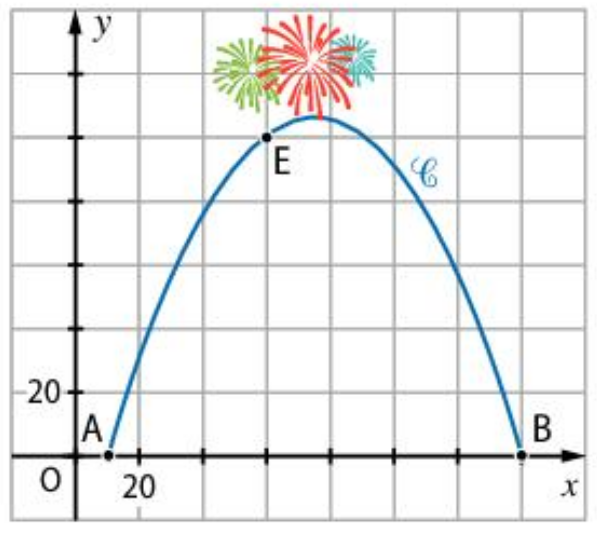
\includegraphics[width=0.35\textwidth]{feu_artifice.png}

%     \begin{enumerate}
%         \item À l'aide du graphique : \begin{enumerate}
%             \item Donner une valeur approchée des solutions de l'équations \(f(x)=0\). À quoi correspondent-elles ?
%             \item Quel est l'ensemble de définition de \(f\) ?
%         \end{enumerate}
%         \item Développer l'expression \((x-10)(x-140)\). Que retrouve-t-on ?
%         \item À l'aide de la réponse précédente, résoudre par le calcul l'équation \(f(x) = 0\).
%     \end{enumerate}
% \end{exo}
\end{multicols}
\end{document}
